\subsection{Battery lifetime}
The battery life of the device was an important factor in state of art section. Thus a tests of the solutions battery life was in order. The tests were set up as follows:
\begin{itemize}
    \item Charge the battery to 100\%.
    \item Connect the wristband to the app.
    \item Disconnect the wristband from power.
    \item Note the time and the battery percentage at a regular interval.
    \item Continue until the device disconnects, or it runs out of battery.
    \item Calculate the battery life from the measured data.
\end{itemize}

This test was repeated 2 times for \textit{some} consistency, though more tests would have been nice to further verify the results.

From the tests \autoref{fig:battery_test_a} and \autoref{fig:battery_test_b},
the battery lasted around 90 minutes. Compared to the mentioned requirement of an entire day, this is comparably low. 
This could be improved with more specific hardware that doesn't draw power for components that aren't used at all, as well as optimizing the code to go in to a low power mode when applicable, and many more power optimizations. For a low-tech prototype of the hardware, the current efficiency is more than satisfactory.

\begin{figure}[H]
  \centering
  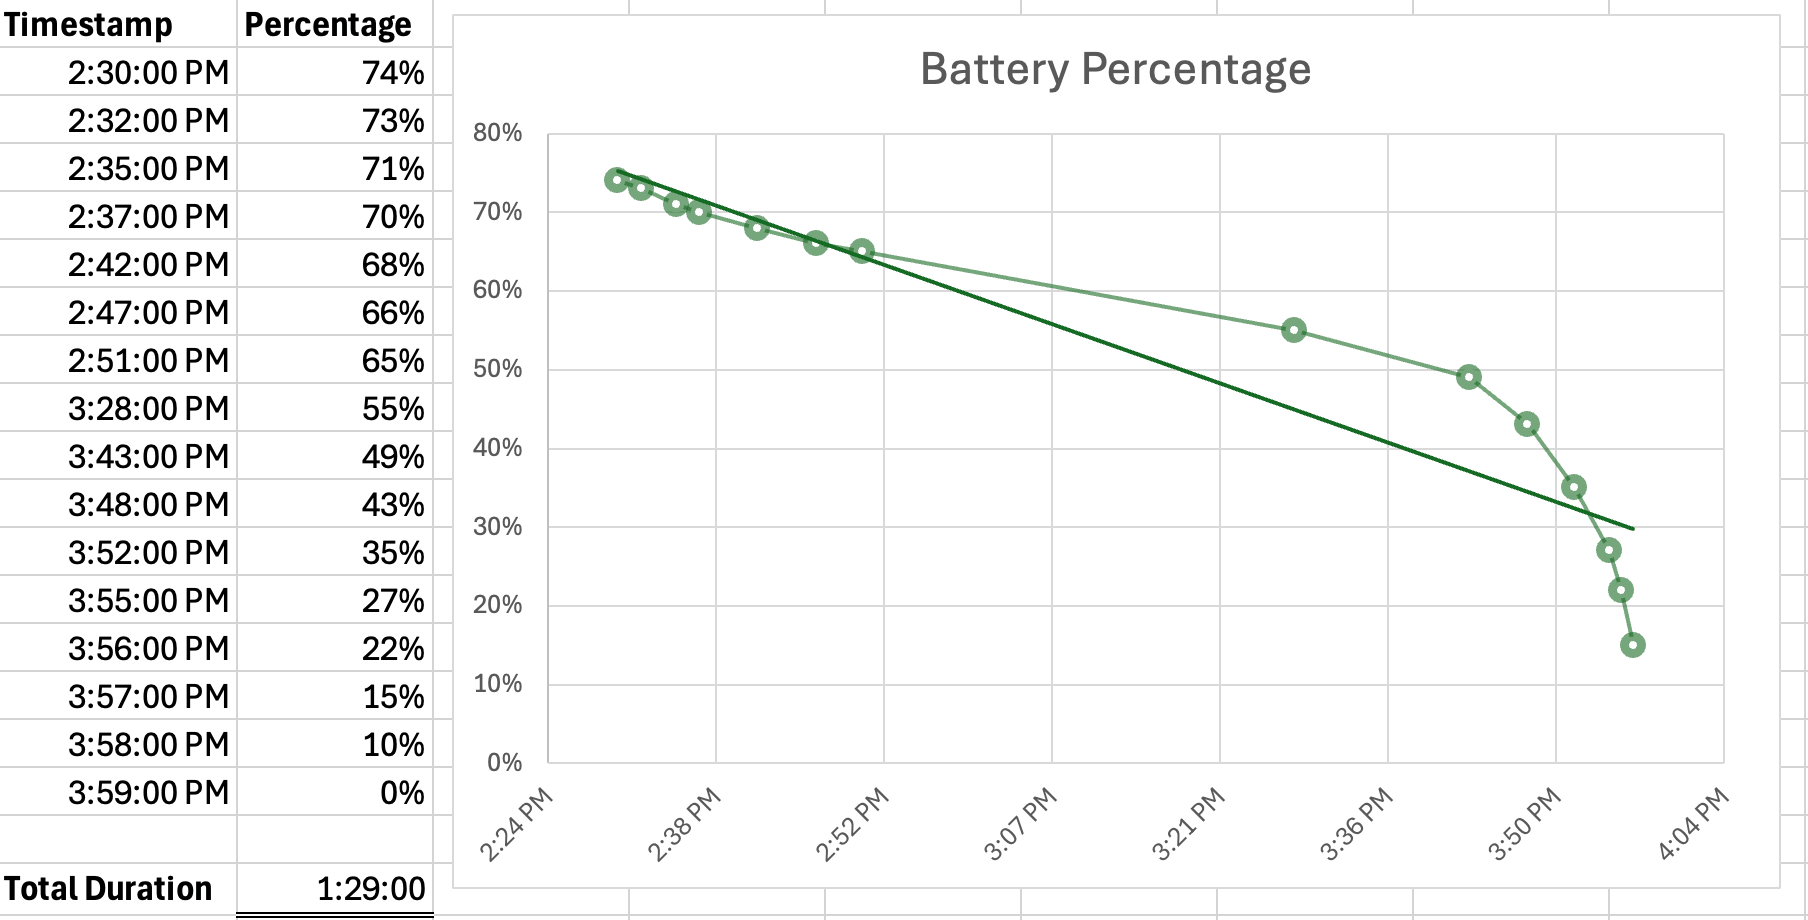
\includegraphics[width=\linewidth]{report/images/Battery Test A.png}
  \caption{Battery percentage over time during the initial battery lifetime test together with a linear regression.}
  \label{fig:battery_test_a}
\end{figure}

Regarding \autoref{fig:battery_test_a}, the percentage column reports 75\% at the start. 
This was verified by measuring the battery voltage, confirming that the battery was fully charged.
The percentage calculation was improved in the later test, although it was not completely corrected.

\begin{figure}[H]
  \centering
  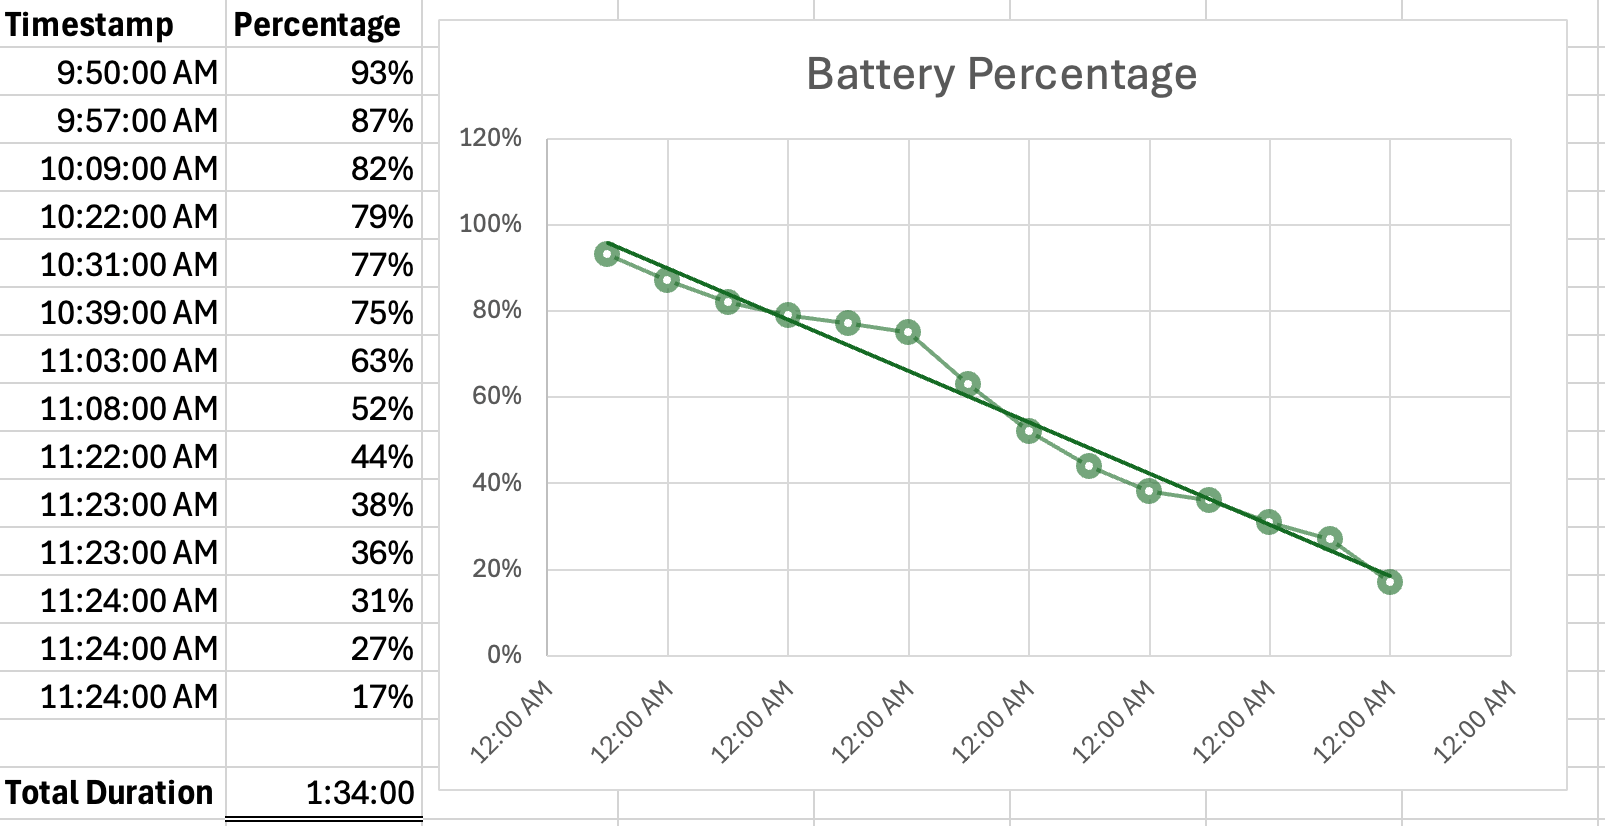
\includegraphics[width=\linewidth]{report/images/Battery Test B.png}
  \caption{Battery percentage over time during the second battery lifetime test together with a linear regression.}
  \label{fig:battery_test_b}
\end{figure}